\chapter{
Integrating Resource Selection with
Spatial Capture-Recapture
  Models}

\markboth{Resource Selection and Space Usage}{}
\label{chapt.rsf}


\vspace{.3in}

Up to this point we have developed many variations of SCR models to
describe the observation process.  These included models of the
relationship between encounter probability and distance, and different
types of covariates such as behavioral responses that can affect
detection probability.  Although these different observation models
are immensely useful, they are rather basic in the sense that they
imply simplistic models of how individuals use space (section
\ref{scr0.sec.implied}) and how individuals are distributed in space.
In the following several chapters we generalize some of the core SCR
assumptions to accommodate more realistic notions of how animals use
space.  


In Sec. \ref{scr0.sec.implied}
we briefly discussed the notion of how SCR encounter probability
models relate to models of space usage.
When we use symmetric and
stationary encounter probability models, SCR models 
imply that space usage is a decreasing function of distance from an
individuals home range center.  In this chapter,
we extend SCR models to incorporate models of resource selection (RS),
such as when one or more explicit landscape covariates are available
which the investigator believes might affect how individual animals
use space within their home range (this is what \citep{johnson:1980}
called {\it third-order} selection).  Our treatment follows
\citet{royle_etal:2012mee} who integrated a standard family of
resource selection models based on auxilliary telemetry data into the
capture-recapture model for encounter probability.  The approach is
consistent with the manner in which classical ``resource selection
function'' (RSF) models \citep{manly_etal:2002} or utilization
distributions \citep{worton:1989, fieberg:2005, fieberg:2007} are
estimated from animal telemetry data.  \citet{royle_etal:2012mee}
argued that SCR models and resource selection models estimated from
telemetry are based on the same basic underlying model of space
usage. The important distinction between SCR and RSF studies are that,
in SCR studies, encounter of individuals is imperfect (i.e.,
``$p<1$'') whereas, with RSF data obtained by telemetry, encounter is
perfect (or, rather, detection is not a {\it stochastic} outcome). We
can think of the two as being exactly equivalent either if we have a
dense array of trapping devices, or if our telemetry apparatus is
imperfect such as only samples a small area of space (this would be
consistent with telemetry stations for sampling fish which only
measure passage).



Telemetry studies are extremely common in animal ecology for studying
movement and resource selection, and SCR studies frequently obtain
such data on a subset of individuals. Thus, formal integration of
capture-recapture with telemetry data for the purposes of modeling
resource selection has a number of immediate benefits. For one, 
 telemetry data provide direct information about $\sigma$
\citep{sollmann_etal:2012ecol,sollmann_etal:inprepjapplecol}. As a
result, this leads to improved estimates of model parameters, and also
has design consequences (see Sec. \ref{design.sec.telemetry}).  In
addition, active resource selection by animals induces a type of heterogeneity in
encounter probability, which is misspecified by standard SCR encounter
probability models. As a result, estimates of population size or
density under models that do not account for resource selection can be
biased \citep{royle_etal:2012mee}.  Finally, because the resource
selection model translates directly to a model for encounter
probability for spatial capture-recapture data, the implication of
this is that it allows us to estimate resource selection model
parameters directly from SCR data, i.e., {\it absent} telemetry
data. This fact should broaden the practical relevance of spatial
capture-recapture for studying or estimating not just density, but
also for directly studyin movement and resource selection.

Telemetry data has been widely 
used in conjuncation with capture-recapture data.  For
example, \citet{white_shenk:2001} and \citet{ivan:2012} suggested
using telemetry data to estimate the probability that an
individual is exposed to sampling. However, their estimator requires that
individuals are sampled in proportion to this unknown quantitiy, which
seems impossible to acheive in many studies. In addition, they do not
directly integrate the telemetry data with the capture-recapture model
so that common parameters are jointly estimated.
\citet{sollmann_etal:inprepjapplecol} and
\citet{sollmann_etal:2012ecol} used telemetry data to directly inform
the parameter $\sigma$ from the bivariate normal SCR model in order to
improve estimates of density, although these models did not include an
explicit resource selection component.



%%% one idea is to use these models to account for sampling along
%%% trails.
%%% define z(x) = trail density or average distance to trail




\section{A Simple Model of Space Usage}
\label{rsf.sec.rsfmodel}

We assume here that our landscape is defined in terms of a discrete
raster of one or more covariates, having the same dimensions and
extent.  Let ${\bf x}_{1},\ldots,{\bf x}_{nG}$ identify the center
coordinates of $nG$ pixels that define a landscape.  We organize these
coordinates into the matrix ${\bf X}_{nG \times 2}$.  Let $z({\bf x})$
denote a covariate measured (or defined) for every pixel ${\bf
  x}$. For clarity, and without loss of generality, we develop the
basic ideas here in terms of a single covariate.  We suppose that a
population of individuals wanders around space in some manner related
to the covariate $z({\bf x})$, and their locations accumulate in
pixels by some omnipotent accounting mechanism. We will define ``use
of ${\bf x}$'' to be the event that an individual animal appeared in
some pixel ${\bf x}$ during some interval of time.

 As a biological matter,
use is the outcome of individuals moving around their home range \citep{hooten_etal:2010},
i.e., where an individual is at any point in time is the result of
some movement process. However, to understand space usage, it is not
necessary to entertain explicit models of movement, just to observe
the outcomes, and so we don't elaborate further on what could be
sensible or useful models of movement, but we imagine existing methods
of hierarchical or state-space
models are suitable for this purpose \citep{jonsen_etal:2005,
  forester_etal:2007, patterson_etal:2008, hooten_etal:2010,
  mcclintock_etal:2012}.
XXX Also cite Ovasakinen papers XXXXXX
We consider explicit movement models in the context of SCR models
later chapters of this book
(Chapt. XXX and XXXX).


If an individual moves from a pixel x to another pixel x' this is
defined as a decision to ``use'' pixel x'. This also induces a
definition of ``truth'' -- that is, over any prescribed time
interval, the animals makes some number, say $R$ of use decisions, and
they are, conceivably, observable by our omnipotent accounting
mechanism (e.g., continuous telemetry).
In this case, 
let $r_{ij}$ be the {\it true} use frequency of pixel $j$ by individual $i$ --
i.e.,
the number of times individual $i$ used pixel $j$.
We assume the 
vector of use frequencies ${\bf r}_{i} = (r_{i1},\ldots,r_{iG})$ has a
multinomial distribution:
\[
{\bf r}_{i} \sim \mbox{Multinom}(R, {\bm \pi}_{i})
\]
where
\[
 \pi_{ij} = \frac{ \exp( \alpha_{2} z({\bf x}_{j}) ) }{ \sum_{x}
   \exp(\alpha_{2} z({\bf x}))}
\]
This is the standard RSF model \citep{manly_etal:2002} used to model
telemetry data.
\hl{One thing about Manly et al 2002 is that they offer
  numerous ways of modeling resource selection. They offer three
  ``protocols'' (pg 5) describing how used and unused resources are
  sampled. What we are discussing is their protocol A where all
  available resources (pixels) are censused, and used pixels are
  sampled randomly for each individual. They also describe 3 designs
  that vary in whether or not individual level data is collected. I
  think it is just worth being aware of this stuff because everybody
  that talks about RSFs thinks in these terms.}
The parameter $\alpha_2$ is the effect of the
landscape covariate $z({\bf x})$ on the relative probability of
use. Thus, if $\alpha_2$ is positive, the relative probability of use
increases as the covariate increases.

In practice, we don't get to
observe $r_{ij}$ for all individuals but, instead, only for a small
subset which we capture and install telemetry devices on.
\begin{comment}
 For these
telemetered individuals we accumulate individual- and pixel-specific
frequencies, at a lower sampling rate than actual individual use. For
example, we might choose to record the location of an individual every
hour or day or whatever. As such, the observed frequency of pixel use
is a {\it sample} of use but, if the recording is random or systematic
(or otherwise unrelated to {\it where} individuals are located), then
we can imagine that the same model of space usage applies. Formally,
we suppose that the observed frequencies are a binomial sample with
sample size $m_{ij}$ and sampling intensity $\phi_{0}$ lets say, and
we see that the constant $\phi_{0}$ cancels from the expression for
the multinomial cell probabilities above.
\end{comment}
For the telemetered individuals, we assume their behavior is according
to the same RSF model as the population as a whole.


We extend this model slightly to make it more realistic spatially. Let
${\bf s}$ denote the centroid of an individuals home range and let
$D_{ij} = ||{\bf x}_{j} - {\bf s}_{i}||$ be the distance from the home
range center of individual $i$, ${\bf s}_{i}$, to pixel $j$, ${\bf
  x}_{j}$. We modify the space usage model to accommodate that space
use will be concentrated around an individuals home range centroid:
\begin{equation}
 \pi_{ij} = \frac{ exp( -\alpha_{1} D_{ij}^{2} +\alpha_{2} z({\bf x}_{j}) ) }
{ \sum_{x} exp(-\alpha_{1} D_{ij}^{2} +\alpha_{2} z({\bf x}_{j}))}
\label{rsf.eq.rsf}
\end{equation}
where $\alpha_1=1/(2\sigma^2)$ describes the rate at which capture
probability declines as a function of distance. This has some context
w.r.t. Johnson et al. and Forester in terms of modeling
``availability'' as a function of distance. But it is not necessary to
distinguish between use vs. availability -- really this model is
cleanly interpreted as individuals using space as a function of how
far away x is from the individuals home range center. Don't see a
need to call that ``availability''.

Note that
Eq.~\ref{rsf.eq.rsf} resembles standard encounter models used in
spatial capture-recapture but with an additional covariate $z({\bf
  x})$ (and see Chapt. \ref{chapt.poisson-mn}).  In particular, under
this model for space usage or resource selection, if you have no
covariates at all, or if $\alpha_{2} = 0$, then the probabilities
$\pi_{ij}$ are directly proportional to the SCR model for encounter
probability.  For example, setting $\alpha_{2} = 0$, then this implies
probability of use for pixel $j$ is:
\[
p_{ij} \propto  \exp( -\alpha_{1} D_{ij}^{2})
\]
so whatever function of distance we use in our RSF implies an
equivalent model of space usage (sec. \ref{scr0.sec.implied}) when
used in SCR models. In particular, for whatever model we choose for
$p_{ij}$ in an ordinary SCR model, we can modify the distance
component in the RSF function in Eq. \ref{rsf.eq.rsf} accordingly to
be consistent with that model, by using whatever function $p_{ij}$ we
choose according to
\[
\pi_{ij} \propto \exp( \log(p_{ij}) + \alpha_{2} z({\bf x}_{j}) )
\]
One difference between this observation model and those that we have
considered in previous chapters is that it includes the normalizing
constant $\sum_{x} \exp(-\alpha_{1} D_{ij}^{2} +\alpha_{2} z({\bf
  x}_{j}))$, which ensures that the use distribution is a proper
probability density function. Thus we are able to characterize the
probability of encounter in terms of both distance and space use.

As an illustration of space usage patterns under this model, we
simulated a covariate that represents variation in habitat structure
(Fig. \ref{rsf.fig.habitat}) such as might correspond to habitat
quality.
\begin{figure}
\centering
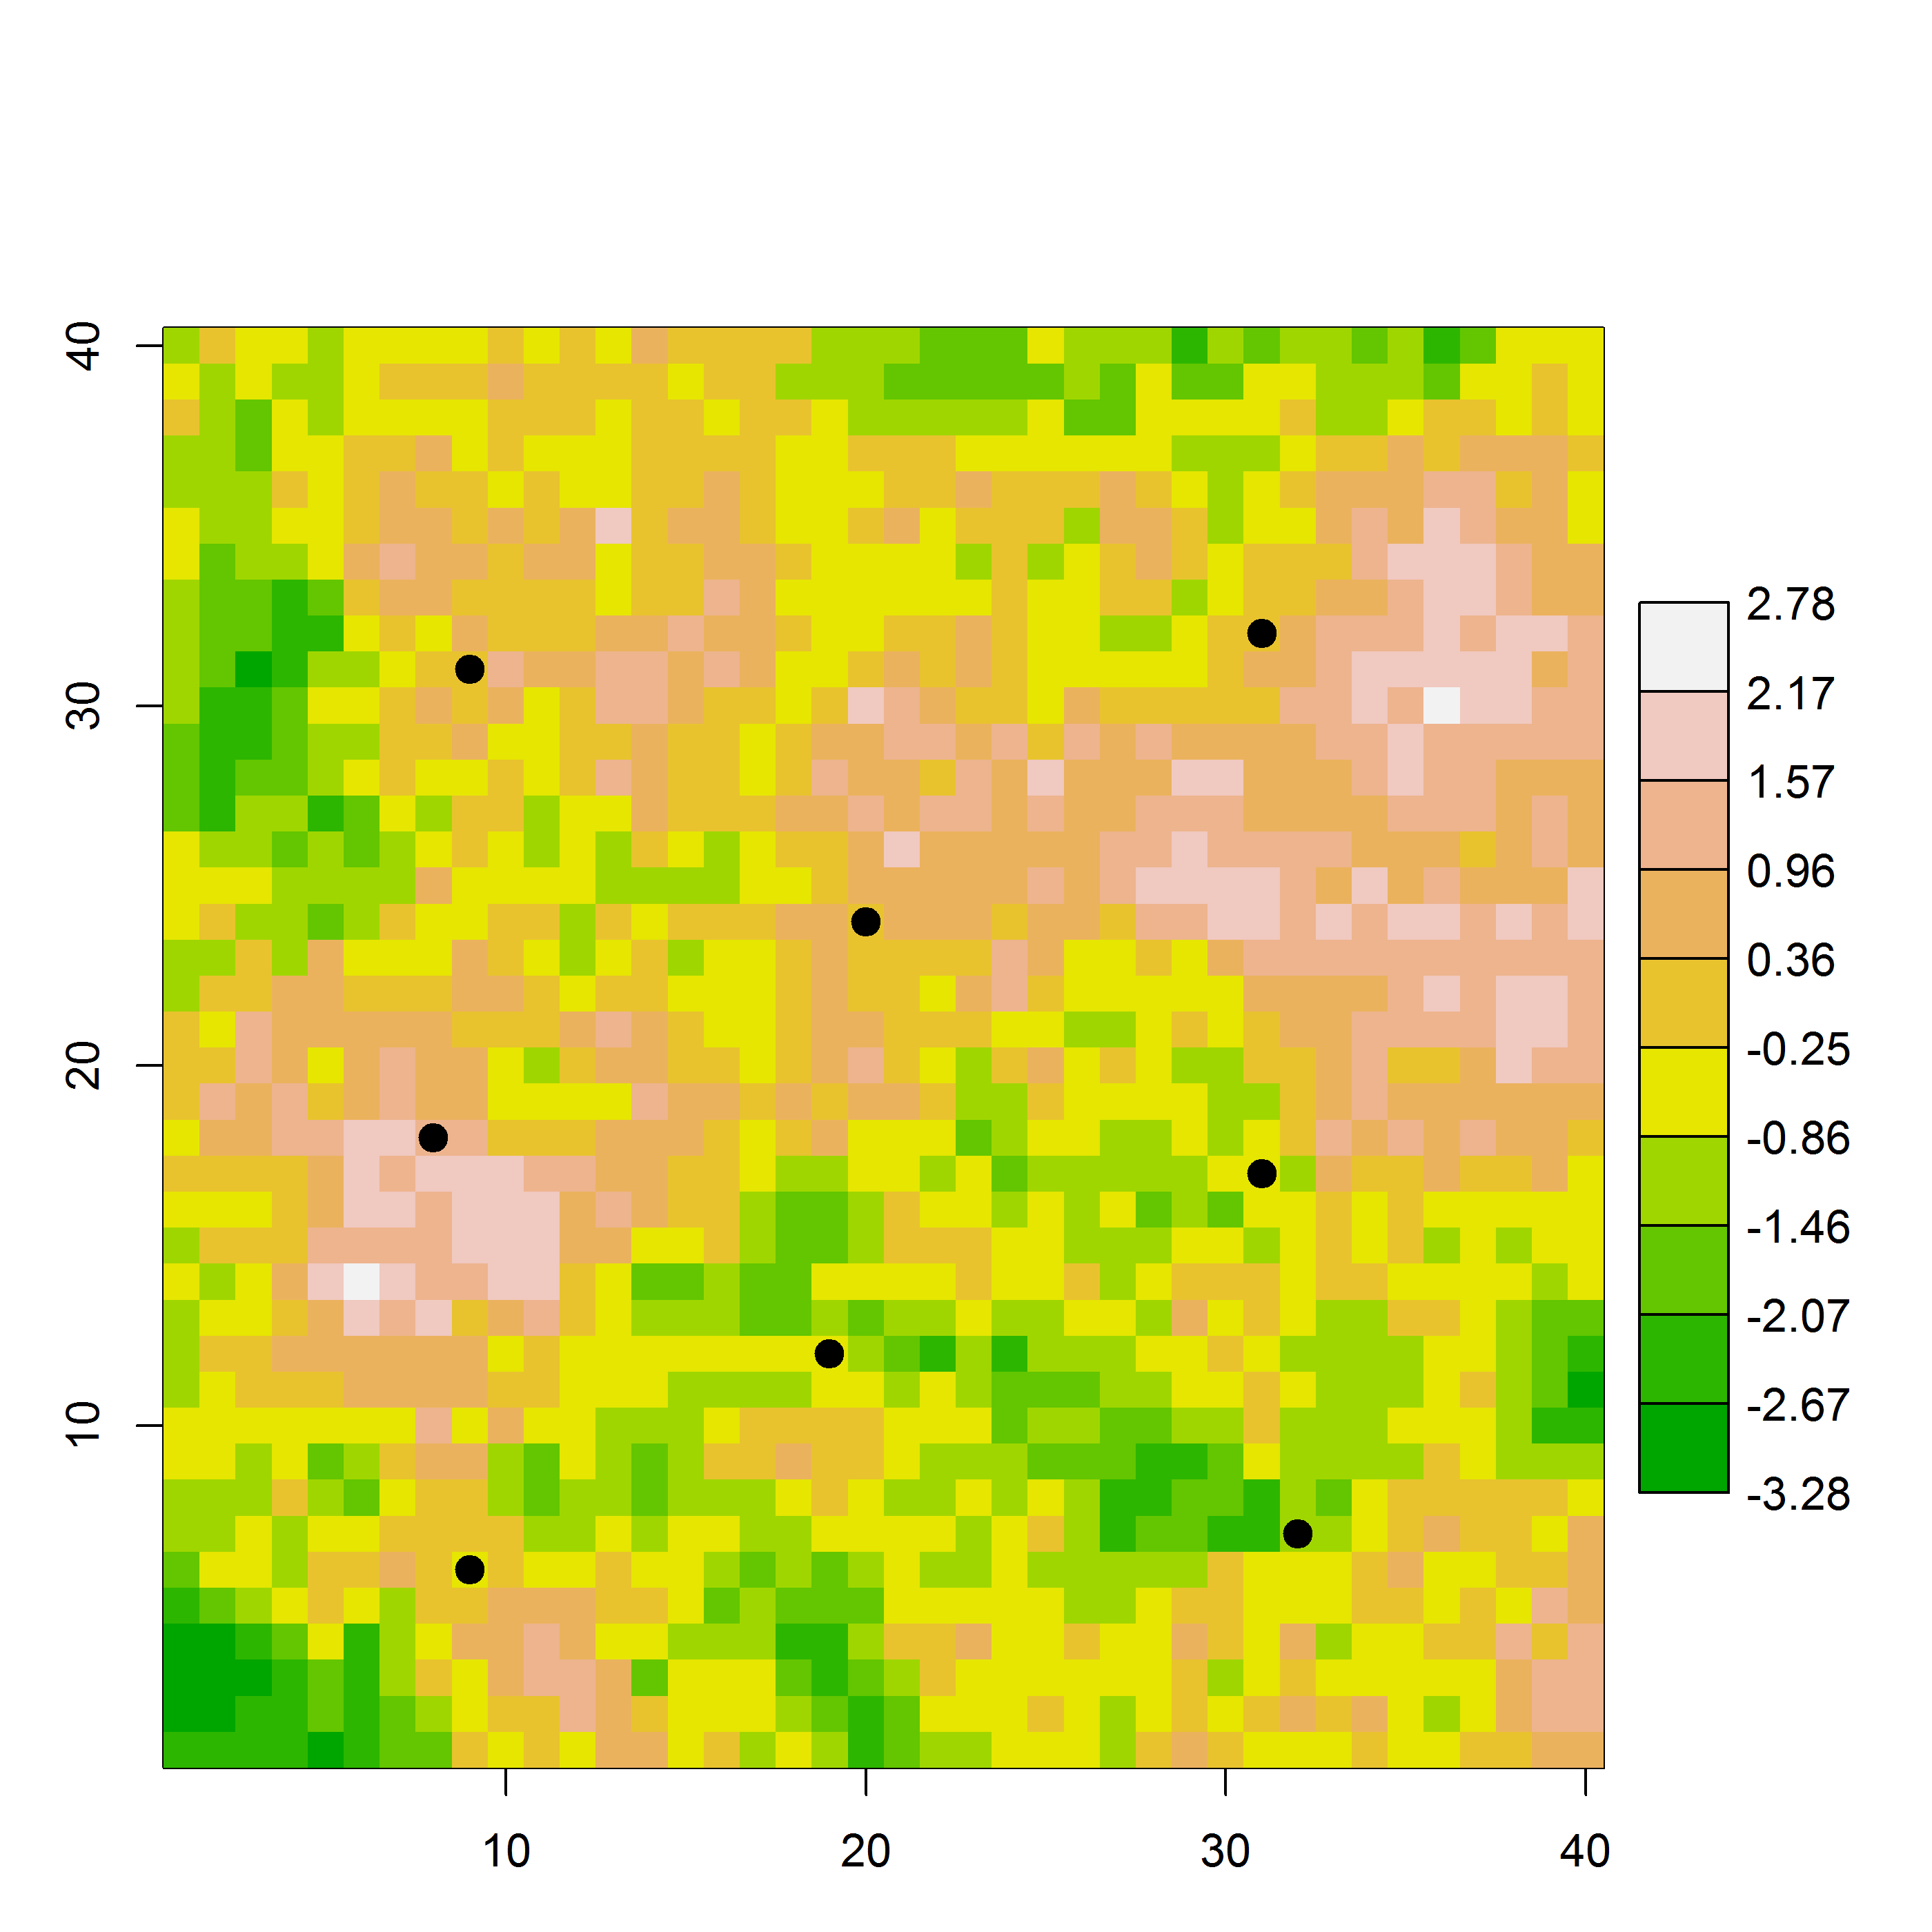
\includegraphics[width=3.5in,height=3.25in]{Ch10-RSF/figs/habitat.png}
\caption{A typical habitat covariate reflecting habitat quality or
  hypothetical utility of the landscape to a species under study. Home range centers for 8 individuals are
shown with black dots.}
\label{rsf.fig.habitat}
\end{figure}
This was simulated by using a
kriging interpolator with the following {\bf R} commands:
\begin{verbatim}
set.seed(1234)
gr<-expand.grid(1:40,1:40)
Dmat<-as.matrix(dist(gr))
V<-exp(-Dmat/5)
z<-t(chol(V))%*%rnorm(1600)
\end{verbatim}
%The functions \mbox{\tt make.statespace} and \mbox{\tt spatial.plot} are
%both in the \mbox{\tt scrbook} package.
Space usage patterns for
 8 individuals are shown in Fig. \ref{rsf.fig.homeranges},
simulated with $\alpha_{1} = 1/(2\sigma^2)$ with $\sigma = 2$ and the
coefficient on $z({\bf x})$ set to $\alpha_{2} = 1$.
\begin{figure}
\centering
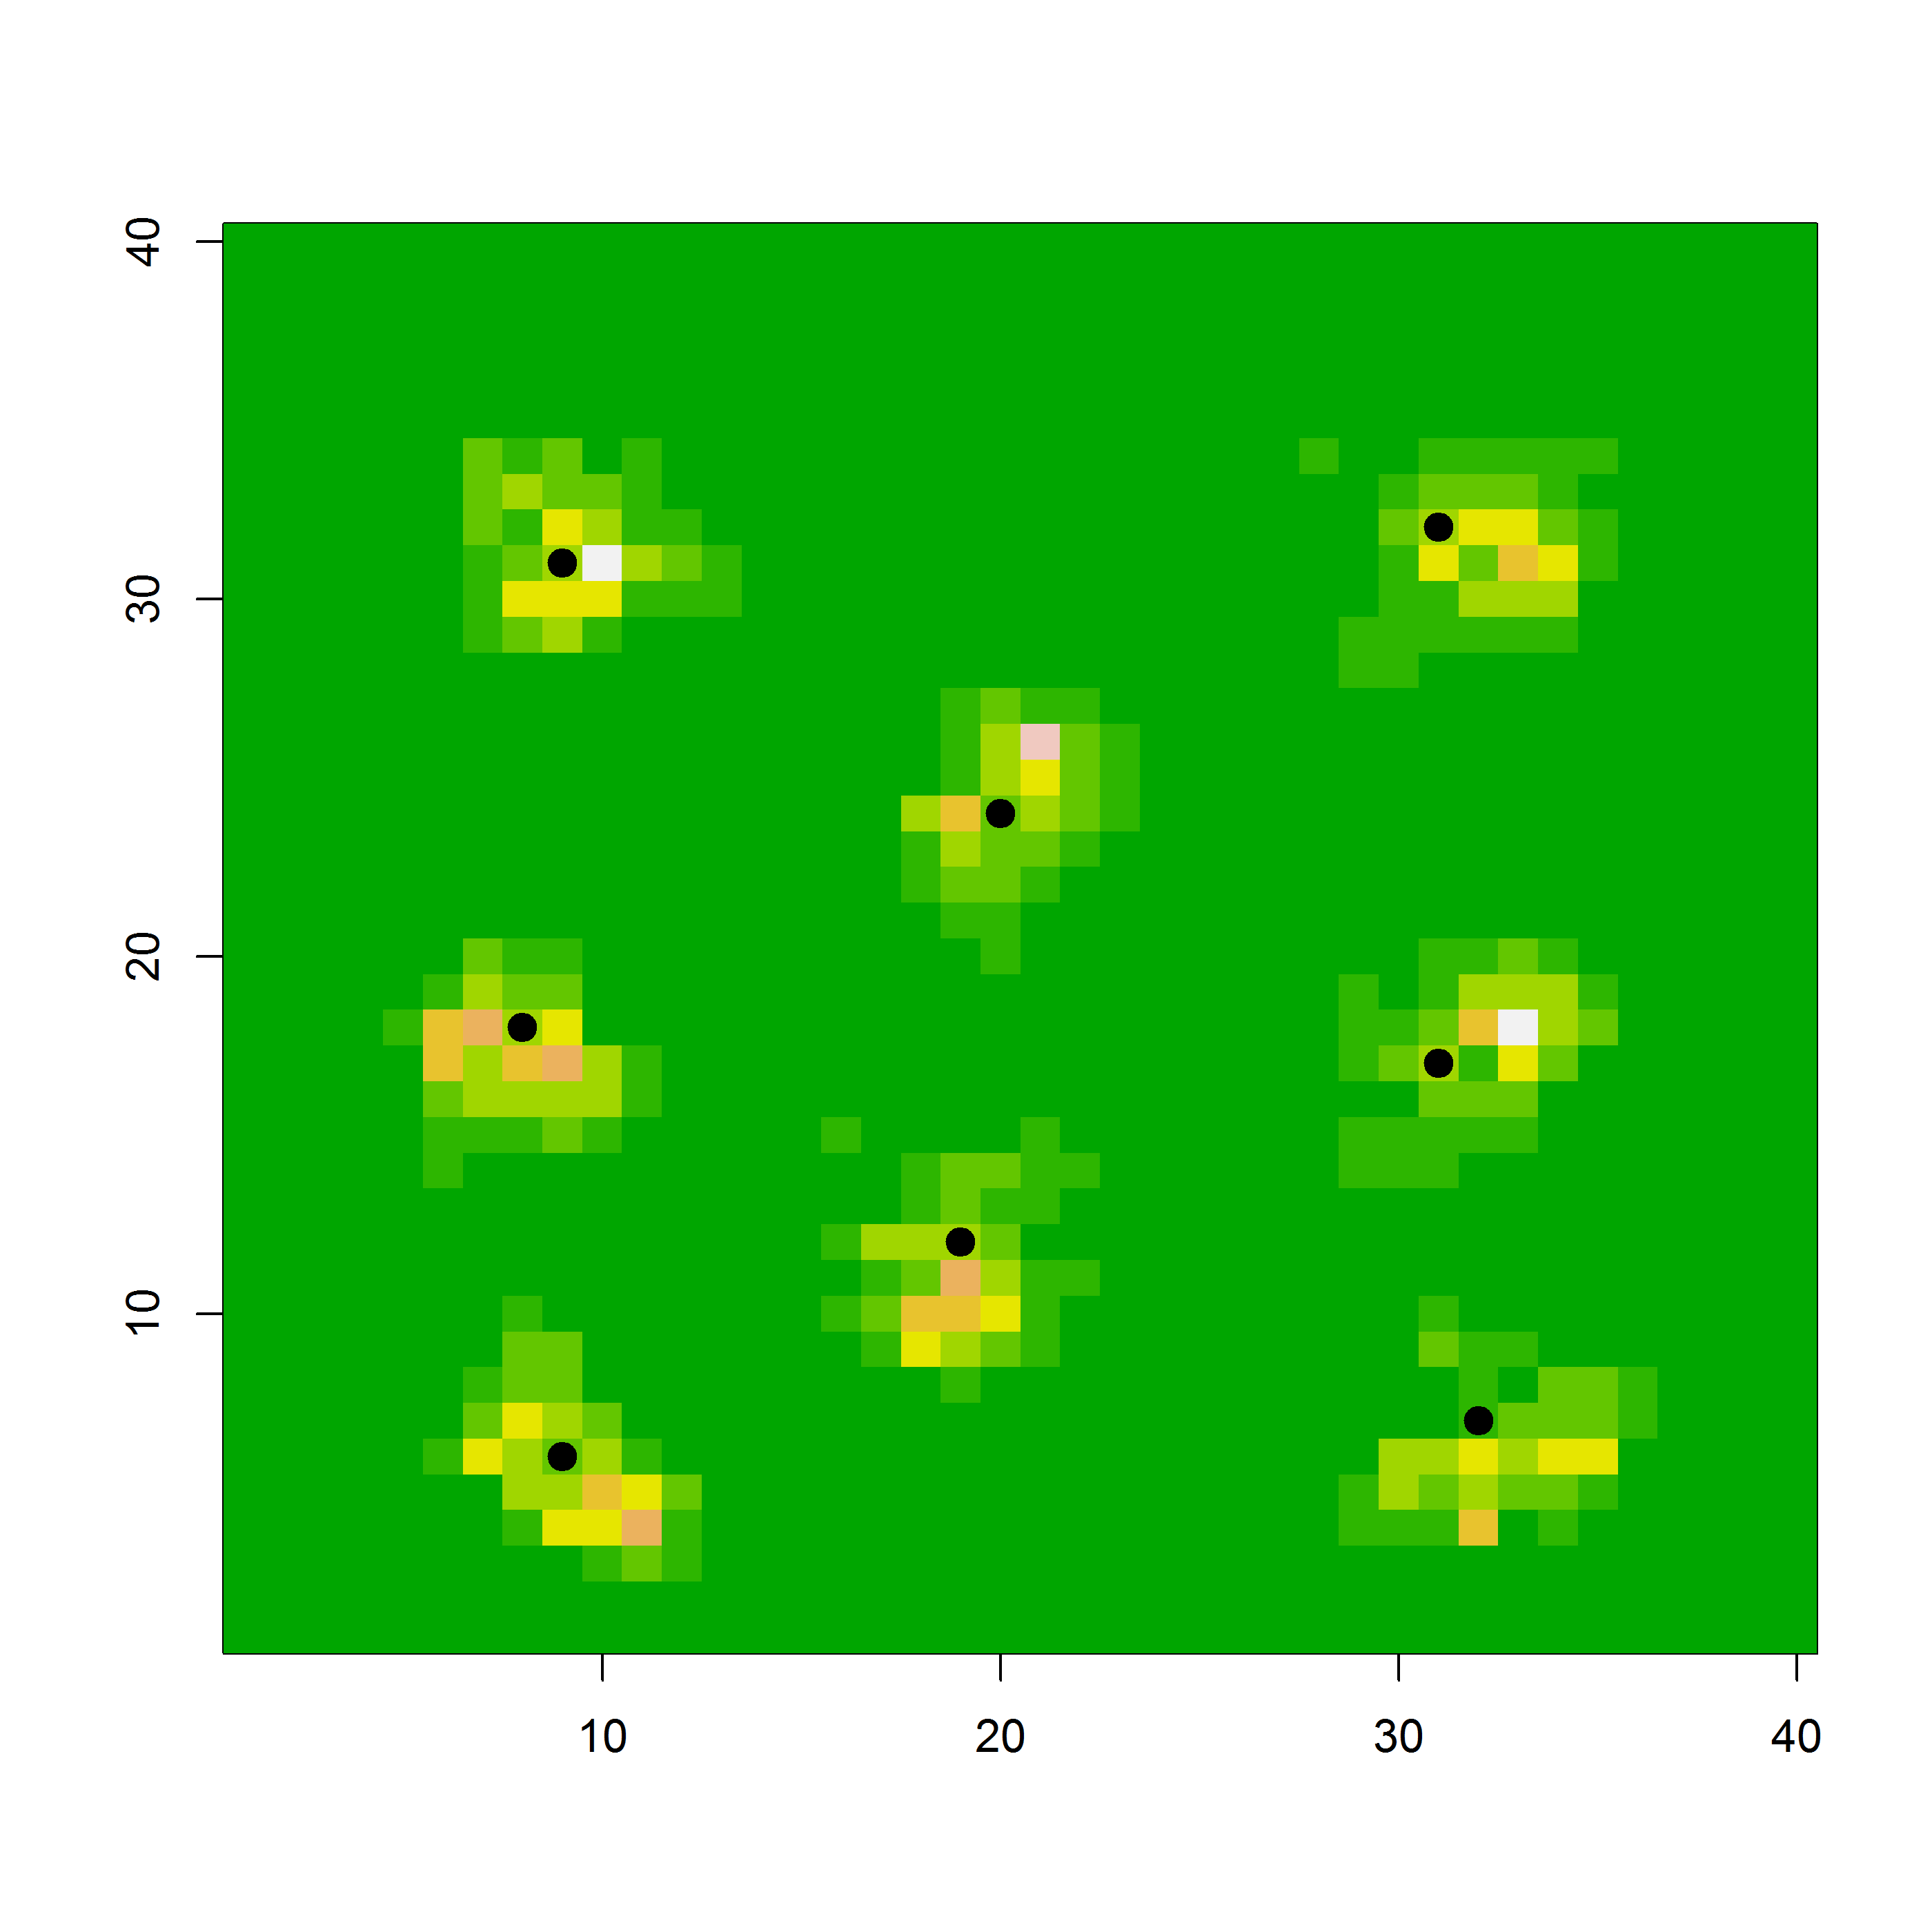
\includegraphics[width=3.5in,height=3.5in]{Ch10-RSF/figs/homeranges8}
\caption{Space usage patterns of 8 individuals under a space usage
  model that contains a single covariate (shown in
  Fig. \ref{rsf.fig.habitat}). Plotted value is the multinomial
  probability $\pi_{ij}$ for pixel $j$ under the model in Eq. \ref{rsf.eq.rsf}.
}
\label{rsf.fig.homeranges}
\end{figure}
These space usage densities -- ``home ranges'' -- exhibit clear
non-stationarity in response to the structure of the underlying
covariate, and they are distinctly asymmetrical.  We note that if
$\alpha_{2}$ were set to 0, the 8 home ranges shown here would
resemble bivariate normal kernels with $\sigma = 2$.  Another
interesting thing to note is that the activity centers are not
typically located in the pixel of highest use or even the centroid of
usage. That is, the observed ``average'' location is not an unbiased
estimator of ${\bf s}$ under the model in Eq. \ref{rsf.eq.rsf}.


\subsection{Poisson use model}

A natural way to motivate the multinomial model of space usage is to
assume that individuals make a sequence of resource selection
decisions so that the outcomes $r_{ij}$ are marginally {\it
  independent}, having a Poisson distribution:
\[
 r_{ij} \sim \mbox{Poisson}( \lambda_{ij})
\]
where
\[
 \log(\lambda_{ij}) = a_{0} -\alpha_{1} D_{ij}^{2} +  \alpha_{2} z({\bf x})
\]
In this case, the number of visits to any particular cell is affected
by the covariate $z({\bf x})$ but has a baseline rate ($\exp(a_{0})$)
related to the amount of movement occuring over some time interval.
This is an equivalent model to the multinomial
model given previously in the sense that, if we condition on the total
sample size $r_{i.} = \sum_{j} r_{ij}$, then the vector ${\bf r}_{i}$
has a multinomial distribution with probabilities
\[
 \pi_{ij} = \frac{\lambda_{ij}}{ \sum_{j} \lambda_{ij}}
\]
which is the same as Eq. \ref{rsf.eq.rsf} (see also
Chapt. \ref{chapt.poisson-mn}) because $a_{0}$ cancels
from the numerator and denominator of the
multinomial cell probabilities
%, analogous to what happens under
%sampling of individual use decisions as discussed above.
and thus this parameter is not relevant to understanding
space usage.

Also note that if use frequencies are summarized over individuals for
each pixel, i.e.,
create the totals $r_j = \sum_i r_{ij}$, then
 a standard Poisson regressino model for the resulting  ``quadrat
 counts'' is reasonable. This is ``Design I'' in \citet{manly_etal:2002}.

\begin{comment}
{\bf note:} while Poisson -> multinomial, it is not vice versa. If the total
sample size per individual is fixed, then the marginals are NOT
Poisson and that model will produce biased estimators.

For purposes of estimation we can use either the Poisson or
multinomial likelihoods. In the former case, we have to estimate an
individual-specific nuisance
parameter $a_{0}$, from which information is derived by the total
number of observations whereas, in the later case, we lose information
about $a_{0}$ by conditioning on the total (i.e., treating it as
fixed).  As it often is fixed, or at least the number of telemetry
observations is completely arbitrary, $a_{0}$ is usually a meaningless
parameter so whether we estimate it or not is immaterial from a
practical standpoint.
\end{comment}





\subsection{Thinning}

Suppose our sampling is imperfect so that we only observe a smaller
number of telemetry fixes than true use, $r_{ij}$. As developed in
sec. \ref{scr0.sec.implied}, we assume that the observed number of
uses is
\[
 m_{ij} \sim \mbox{Bin}(r_{ij}, \phi_{0}).
\]
We can think of these countas as arising by thinning the underlying
point process (here, aggregated into pixels) where $\phi_{0}$ is the
thinning rate of the point process.
In this case, the marginal distribution of $m_{ij}$ is also Poisson
but with mean
\[
 \log(\lambda_{ij}) = \log(\phi_{0}) + a_{0} -\alpha_{1} D_{ij}^{2} +  \alpha_{2} z({\bf x}).
\]
Thus, the space-usage model (RSF) for the
thinned counts $m_{ij}$ is the same as the space-usage model for the
original variables $r_{ij}$.  This is because if we remove $r_{ij}$
from the conditional
 model by summing over its possible values, then the vector of
${\bf m}_{i}$ is {\it also}  multinomial with cell probabilities
\[
\pi_{ij} = \frac{\phi_{0}\lambda_{ij}}{\sum_{j} \phi_{0} \lambda_{ij}}
\]
and so the nuisance parameter $\phi_{0}$ cancels from the numerator and
denominator. Thus, the underlying RSF model applies to the true
unobserved count frequencies ${\bf r}_{i}$ and also those produced
from thinning or sampling, ${\bf m}_{i}$.

%KEY POINT LOST HERE IS THAT BOTH TELEMETRY AND SCR ARE RANDOMLY
%THINNED VERSIONS OF THE POINT PROCESS, PROVIDED CAMERA TRAPPING IS
%RANDOM ALSO

In summary, if we conduct a telemetry study we observe ${\bf r}_{i}$,
the $nG \times 1$ vector of pixel-counts for each individual
$i=1,\ldots,N_{tel}$.  We declare these data to be
``resource-selection data'' which are typical of the type used to
estimate resource-selection functions (RSFs) \citep{manly_etal:2002}.
Sometimes in RSF modeling activities we might have
continuous covariates and so the denominator in Eq. \ref{rsf.eq.rsf}
involves an integration over a distribution for the covariate which is
the conditional intensity of observed point locations in a point
process model. However, in a discrete landscape, entertaining pdfs for
the covariates isn't necessary \citep{royle_etal:2012mee} when we
recognize that the denominator should be the expectation over {\it
  space} and not the pdf of some covariate.


\subsection{Capture-recapture Data}

XXXXXXXXXXXXXXXXXXX
RC says: After reconciling SCR and RSF, cite that paper
by Boyce and McDonald where they try to do accomplish the same
objective using ad-hoc methods. That is the only effort to do
something similar that I am aware of.
XXXXXXXXXXXXXXXXXXXXXXXXXX

The key to combing RSF data with SCR data is to work with this
underlying resource utilization process and formulate SCR models in
terms of that process. The idea in \citep{royle_etal:2012mee} was to
define the true use frequency for each pixel as 
the intermediate latent variable to which both telemetry data and SCR
data are linked.
Obviously we have to assume that both telemetered individuals
and SCR individuals are using space according to the same resource
selection model. The difference is that, for SCR data, we do not have
sampling devices in all locations (pixels) in the landscape, and hence
the data are only recorded at a subsample of them. XXXXX {\bf move the
  following } XXXXX
In other words,
imagine that we have a sampling device, such as a camera trap, in {\it
  every} pixel. If the device operates continually then it is no
different from a telemetry instrument.  If it operates intermittently
and does not expose the entire area of each pixel then a reasonable
model for this imperfect observation is the ``thinned'' binomial model
given above, where $\lambda_{0} \equiv \exp(\phi_{0})$ represents the
sampling effectiveness of the device. So we imagine that the
hypothetical perfect data from a camera trapping study are the thinned
counts $m_{ij}$ for every pixel $j$.

Introducing the latent use
 frequencies $m_{ij}$, and considering the Bernoulli SCR model
where
$y_{ij} = 1$  if the individual $i$ visited the pixel
containing a trap and was detected, then
we imagine that $y_{ij}$ is related to the latent variable $m_{ij}$ being the
event $m_{ij}>0$, which occurs with probability
\[
 p_{ij} = 1-\exp(- \lambda_{ij})
\]
where
\[
 \log(\lambda_{ij}) = \log(\phi_{0}) + a_{0} -\alpha_{1} D_{ij}^{2} +  \alpha_{2} z({\bf x}).
\]
We combine the constants so that $\alpha_{0} = \log(\phi_{0}) + a_{0}$
is the baseline encounter rate which includes the constant intensity
of use by the individual and also the baseline rate of detection,
conditional on use.  The Bernoulli observation model implies that the
observed encounter frequencies for individual $i$ and trap $j$, from
sampling over $K$ encounter periods is:
\[
 y_{ij}|{\bf s}_{i} \sim \mbox{Bin}(K; p_{ij})
\]
We imagine that any of the standard SCR observation model could be
implemented here with only minor modifications of the encounter
probability model (following the developments of Chapt. \ref{chapt.poisson-mn}.


\section{The Joint RSF/SCR Likelihood}

To construct the likelihood for SCR data when we have auxiliary
covariates on space usage {\it or} direct information on space usage
from telemetry data, we regard the two samples (SCR and RSF) as
independent of one another. In practice, this might not always be the
case but (1) often time the telemetry data come from a previous study;
(2) the individuals are not the same at all; (3) or even if they are
some of the same individuals being captured, we might not be able to
match individuals captured by a sampling method such as hair-snares
with the individuals wearing radio-collars; (4) In cases where we {\it
  can} match some individuals between the two samples, regarding them as
independent should only entail a minor
loss of efficiency
because we are disregarding more precise information on a small number
of activity centers. Moreover, we believe, it is unlikely in practice
to expect the two samples to be completely reconcilable and that the
independence formulation is the most generally realistic.

Regarding the two data sets as being independent, our approach here
is to form the likelihood for each set of observations as a function
of the same underlying parameters and then combine them. In
particular, let ${\cal L}_{scr}(\alpha_{0}, \alpha_{1}, \alpha_{2}, N;
{\bf y}_{scr})$
be the likelihood for the SCR data in terms of the basic encounter
probability parameters and the total (unknown) population size $N$,
and let ${\cal L}_{rsf}(\alpha_{1},\alpha_{2}; {\bf m}_{rsf})$ be the
likelihood for the RSF data based on telemetry which, because the
sample size of such individuals is fixed, does not depend on $N$.
Assuming independence of the two datasets, the
joint likelihood is the product of these two pieces:
\[
{\cal L}_{rsf+scr}(\alpha_{0},\alpha_{1},\alpha_{2},N; {\bf y}_{scr},{\bf
  m}_{rsf})  = {\cal L}_{scr} \times {\cal L}_{rsf}
\]
In what follows, we provide a formulation of each likelihood
component, along with an {\bf R} function for obtaining the MLEs of
model parameters using standard methods available in {\bf R}.


Where the L(scr) is the normal integrated likelihood (chapt XXX,
equation XXXX) and the rsf likelihood is the multinomial telemetry
likelihood from eq. XXXX above. 
That is, if we estimate s for the telemtered guys by the mean location
then we could use that plug-in otherwise we also have to inegrate the
multnomial likelihood ..........
For the RSF data from the sample of individuals with telemetry devices
we adopt the same basic strategy of describing the
conditional-on-${\bf s}$ likelihood and then computing the marginal
likelihood by averaging over possible values of ${\bf s}$.
We have ${\bf m}_{i}$, the vector of pixel counts for individual $i$,
where these counts are derived from a telemetry study or similar.
The conditional-on-${\bf s}_{i}$ distribution of the telemetry data
from individual $i$ is:
\[
 [{\bf m}_{i}  | {\bm \alpha} ]
 = \prod_{g=1}^{G}  \pi_{ij}({\bf s}_{i},z({\bf x}_{j})) ^{r_{ij}}
\]
where
\[
 \pi_{ij}  = \frac{ \exp( -\alpha_{1} D_{ij}^{2} +\alpha_{2} z({\bf x}_{j}) ) }
{ \sum_{g} \exp(-\alpha_{1} D_{ij}^{2} +\alpha_{2} z({\bf x}_{j}))}
\]
The marginal pmf is:
\[
     [{\bf m}_{i}|{\bm \alpha}] =    \int_{{\cal S}}  [ {\bf m}_{i} |{\bf s}_{i},{\bm \alpha}] g({\bf s}_{i}) d{\bf s}_{i}
\]
and therefore the likelihood for the RSF data is
\[
{\cal L}_{rsf}({\bm \alpha} | {\bf m}_{1},{\bf m}_{2},\ldots, {\bf m}_{Ntel}) = \prod_{i=1}^{Ntel}
[{\bf m}_{i}|{\bm \alpha}].
\]

An R script is given in \mbox{\tt scrbook} which is the function XXXX
from manuscript ADD TO REPO XXXXXX... will handle estimated s by sbar
or whatever.   Should be obvious that estimating s with sbar is not
the greatest thing because there is a covariate affecting use, and so
we expect the geographic centroid to be biased for s.



\section{Application: New York Black Bear Study}
\label{rsf.chapt.nybears}


\citet{royle_etal:2012mee}
applied the integrated SCR+RSF model to data from a study of black bears in a
region of approximately 4,600 km$^2$ in southwestern New York
\citep{sun:2013}. We reproduce their results here.
The data can be loaded from the \mbox{\tt scrbook} library with the
command \mbox{\tt data(nybears)}. {\bf XXXX do this on the repo XXXXX}
A noninvasive, genetic, mark-recapture
study was conducted to estimate density, and a concurrent telemetry
study was conducted in the same study area to understand patterns of
landscape connectivity and space usage.
The study used DNA sampling obtained from 103
hair snares 
(Fig. \ref{rsf.fig.studyarea})
set  from 6 June - 9 July, 2011.
Hair snares
were baited and scented and checked weekly for hair. 
See \citet{sun:2013} for details of the genetic analysis.

The study yielded
captures of 33 individuals and a total of 14 recaptures (27
individuals captured 1 time only; 3 individuals captured twice; 1
individual each three and four times). Extra trap recaptures included
3 individuals captured in 2 traps, 1 individual in each of 3 and 4
traps.  We used data from 3 radio-telemetered individual bears (2M,
1F) from the same time period as the SCR data. Radio fixes were
obtained approximately once per hour and a total of 1,948 fixes on the
3 individuals were obtained. We thinned these hourly fixes to once per
10 hours to approximate the data as independent movement outcomes,
producing 195 telemetry locations used in the RSF component of the
model.  We used the covariate elevation in the model, derived from a
one arc-second digital elevation model (USGS National Elevation
Dataset, accessed June 2012).  This is shown in
Fig. \ref{fig.elevation} (on a
standardized scale) which also shows the locations of each capture
(multiple captures at a trap location are dithered by adding random
noise).


We fitted a sequence of models based on the Gaussian hazard model
(eq. \ref{eq.hazard})  including an ordinary SCR model with no
covariates or telemetry data, the SCR model with elevation affecting either
$\lambda_{0}$ or density $D({\bf x})$, and models that use telemetry data. We have not discussed modeling
covariate effects on density, but such models are described by
\citet{borchers_efford:2008} and we have not provided any novel
treatment of that modeling aspect here.
The full list of models (with labels) is as follows:
\begin{itemize}
\item[] Model 1: SCR -- ordinary SCR model
\item[] Model 2: SCR+p(z) -- ordinary SCR model with elevation as a
  covariate on baseline encounter probability $\lambda_{0}$.
\item[] Model 3: SCR+D(z) -- ordinary SCR model with elevation as a
  covariate on density only.
\item[] Model 4: SCR+p(z)+D(z) -- ordinary SCR model with elevation as
  a covariate on both baseline encounter probability and density.
\item[] Model 5: SCR+p(z)+RSF -- SCR model including data from 3
  telemetered individuals.
\item[] Model 6: SCR+p(z)+RSF+D(z) -- SCR model including telemetered
  individuals and with elevation as a covariate on density.
\end{itemize}
The first 4 models can be viewed together for purposes of
model-selection by AIC since they are nested models. The last two
models can be viewed together but cannot be compared to the first 4
because they include telemetry data.
The results of fitting these 6 models -- the parameter estimates and
standard errors are shown in Table \ref{tab.nyresults}.
We provide a full R script for fitting  all of these models to
simulated data in Appendix 1.


Among models 1-4, those models {\it without} the telemetry data, we
see that the two models with elevation affecting density are preferred
-- and, there is a large positive response to elevation. This is
consistent with the visual pattern apparent in
Fig. \ref{fig.elevation} where we see individual captures favoring
high elevation sites.  We also see a negative effect of elevation on
{\it space usage} (the parameter $\alpha_{2}$).  It is interesting
that the sign of the estimate of $\alpha_{2}$ changes from positive to
negative when we add elevation as a covariate on density. Thus, the
effect of elevation on density appears to have masked its effect on
space usage.  The estimate of $N$ for the 4600 km$^2$ state-space is
about 103 bears $(\exp(4.25)+33)$.

In the two models that include the additional telemetry data, a couple
points stand out: Clearly the elevation effect on density is
important, reducing the negative log-likelihood by 5 units. The effect
of elevation on density and space usage are roughly consistent with
Model 4 which did not use telemetry data. Furthermore, the standard
errors (SE) of those two parameter estimates are reduced considerably
when the model uses telemetry data, as is the SE for estimating
$\log(\sigma)$.  The SE for estimating $\log(n_{0})$ is only improved
incrementally compared to the models without telemetry data.  We used
the best model, \mbox{\tt SCR+p(z)+RSF+D(z)}, to produce a map of
density (Fig. \ref{fig.density}) which shows clearly the pattern
induced by elevation. We also produced a map
(Fig. \ref{fig.spaceusage}) to illustrate the effect of elevation on
space usage. This shows the relative probability of using a pixel
${\bf x}$ relative to one of mean elevation, and of the same distance
from an individual's activity center.
% remind people how to compute "the relative prob of using pixel x XXXX
%The cool thing about these models is we can make pretty
%multi-colored maps of things.  A map of density under the 
%model is shown in fig. \ref{fig.density}.  A map of space usage in
%terms of the relative probability of using pixel $x$ relative to the
%average pixel is shown in Fig. \ref{fig.spaceusage}.


% XXXX should we add AIC to this table? XXXX
\begin{table}
\centering
\caption{
Summary of model-fitting results for the black bear study. Parameter
estimates are $\alpha_{0} = \log(\lambda_{0})$ and $\sigma$ is the
scale parameter of the half-normal hazard rate encounter model.
The SCR data are based on $n=33$ individuals, and the telemetry data
are based on 3 individuals.
}
\begin{tabular}{c|rrrrrr}
\hline \hline
model & $\alpha_0$ & $\log(\sigma)$ & $\alpha_{2}$ & $\log(n_{0})$ &
$\beta$ & -loglik \\ \hline
SCR+p(z)     & -2.8600  & -1.1170  &  0.1750 &  4.1400   &        &122.7380  \\
   SE        &  0.3899 &  0.1390 &  0.2478&  0.3657  &        & \\
 SCR         & -2.7290  &  -1.1220 &  ---&  4.1100   &        &              122.9900   \\
   SE        &  0.3454 &   0.1404&        &  0.3618  &        &       \\
SCR+D(z)     & -2.7150  & -1.1330  &  ---  &  4.1140   & 1.2470  &   118.0070  \\
   SE        &  0.3526 & 0.1394  &        &  0.3575  & 0.4083 &       \\
SCR+p(z)+D(z)& -2.4840  & -1.1570  &-0.3840  &  4.2550   & 1.5710  &      117.0750 \\
   SE        &  0.3910 &  0.1421 & 0.2761 &  0.3768  & 0.4630 & \\
SCR+RSF     &   -3.0680  & -0.8140  &-0.2810  &  3.8840   &        &   1271.7390 \\
   SE       &    0.2722 &  0.0364 & 0.1176 &  0.3626  &        & \\
SCR+RSF+D(z)&  -3.0700  &-0.8100   &-0.3710  &  4.0280   & 1.2730  &   1266.7000 \\
   SE       &   0.2720 &  0.0368  & 0.1239 &  0.3661  & 0.4110 &    \\
\hline
\end{tabular}
\label{tab.nyresults}
\end{table}





Resource selection can be described in
hierarchical orders \citep{johnson:1980}, from selection of a geographical
area (first-order selection), selection of a home range within a study
area (second-order), or selection of resources with that home range
(third-order).  Animals may select resources at different scales as a
result of variability in the distribution of resources on the
landscape \citep{mayor_etal:2009}.  Indeed, black bears make habitat
selection decisions at multiple spatial scales, and decisions made at
the second-order can differ from those at the third-order
\citep{lyons_etal:2003, sadeghpour_ginnett:2011}.
  As a result of multi-scale
resource selection, we can expect that the modeled covariates
(elevation in our example) may affect density and space usage
differently.  We suggest that density is operating at the second-order
and is largely related to the spacing of individuals and their
associated home ranges across the landscape.  On the other hand, our RSF was defined
based on selection of resources within the home range (third-order).
Because density and our third-order RSF were at different spatial
scales, there is no expectation that the modeled covariate describing
space usage (elevation) would influence each in a similar manner.
Consistent with our positive relationship between elevation and
density, the distribution of a black bear population in the central
Appalachian Mountains was positively associated with elevation \citep{frary_etal:2011}.
 At the second-order, however, we observed a negative
effect of elevation on space usage.  Our study was conducted during
summer, and seasonal shifts in elevation have been widely documented
in black bears, often attributed to seasonal variation in food
availability \citep{reynolds_beecham:1980,
%garshelis_pelton:1981,kendall:1983, 
graber_white:1983}.
%%irwin_hammond:1985, raine_kansas:1990}.
 The negative relationship between elevation and space
usage during the summer could be attributable to either access to food
resources at lower elevations, or access to river and stream
corridors.  Within their home ranges, black bears selected areas with
high stream densities \citep{fecske_etal:2002}, and in our study area,
lower elevations were associated with river corridors which likely
provided bears cooler conditions during the heat of summer.





\section{Simulation Study}

Royle et al. XXXXX 
 carried-out a simulation study using the landscape shown in
Fig. \ref{rsf.fig.habitat}, and based on a population of $N=100$ and $N=200$
individuals with activity centers distributed uniformly over the
landscape.  This patchy covariate was simulated by generating a field
of spatially correlated noise to emulate a typical patchy habitat
covariate such as tree or understory density, or some other covariate
relevant to habitat quality for a species.  We subjected individuals
to sampling over $K=10$ sampling periods, using a $7 \times 7$ array
of trapping devices located on the the integer coordinates $(u*5,v*5)$
for $u,v = 1,2,3,4,5,6,7$. The model parameters were
\[
\mbox{ cloglog}(p_{ij}) = -2  -\frac{1}{2\sigma^{2}} D_{ij}^{2} + 1 \times z({\bf x}_{j})
\]
for $\sigma =2$. In the absence of the covariate $z$, this corresponds
to an individual having a bivariate normal home range with standard
deviation 2.
These settings yielded an average of about $n=61$ individuals captured for
the $N=100$ case and about $n=123$ for the $N=200$ case. The later case
represents what we believe is an extremely large sample size based on
our own experience and thus it should serve to gauge the large sample
bias of the likelihood estimator (note: we expect little to no large
sample bias).

In addition to simulating data from this capture-recapture study, we
simulated 2, 4, 8, 12, 16 telemetered individuals to assess the
improvement in precision as sample size increases.  For all cases we
observed 20 telemetry fixes {\it per} individual.  The main things
we're focused on with this simulation study were: (1) how much does
the SE of estimated $N$ improve as we add or increase the number of
telemetered individuals?  (2) How well does the SCR model do at
estimating the parameter of the RSF with {\it no} telemetry data?  (3)
How much does the precision of the RSF parameter improve if we add SCR
data to the telemetry data?


%% Should also simulate fitting the wrong model with symmetric
%% encounter model and see what happens
%% also run N=200 with 500 iterations

{\small
\begin{verbatim}
N=100, 300 iters each, mean SCR only N: 99.418     N=200, 500 iters. Mean SCR only N = 199.712
n=2          Nhat RMSE  ahat RMSE  sighat  RMSE    Nhat RMSE  ahat RMSE  sighat  RMSE
SCR only:   99.73  9.97  0.99  0.14  2.00  0.124  198.85  14.24   0.99   0.10   2.00   0.091
SCR/RSF:    99.94  9.54  0.99  0.12  2.00  0.097  199.37  12.80   0.99   0.09   2.00   0.078
sbar        98.89  9.50  0.93  0.14  1.97  0.100  197.87  13.94   0.96   0.10   1.99   0.080
RSF only     --    --    1.03  0.33  2.00  0.160    --      --    1.04   0.33   1.99   0.169
n=4
SCR only    99.10  9.83  0.99  0.13  2.00  0.127  200.06  15.34   1.00   0.09   2.00   0.092
SCR/RSF     99.17  9.47  0.99  0.11  2.00  0.086  200.25  14.36   1.00   0.08   2.01   0.073
sbar        97.43  9.68  0.89  0.16  1.97  0.090  198.14  14.31   0.94   0.10   1.98   0.075
RSF only     --     --   0.98  0.22  2.00  0.119    --     --     1.02   0.21   2.01   0.122
n=8
SCR only    99.59 10.00  1.00  0.13  2.00  0.130  200.85  14.06   1.00   0.09   2.00   0.087
SCR/RSF     98.90 10.02  0.99  0.10  2.00  0.071  200.29  13.98   1.00   0.08   2.00   0.061
sbar        96.07 10.37  0.84  0.19  1.96  0.078  196.46  14.59   0.90   0.13   1.97   0.069
RSF only     --    --    0.98  0.16  2.01  0.084    --     --     0.99   0.16   2.00   0.084
n=12
SCR only    99.44 10.73  0.98  0.13  2.02  0.128  198.76  14.47   0.99   0.10   2.00   0.091
SCR/RSF     99.96 10.26  1.00  0.09  2.00  0.059  198.72  14.14   1.00   0.08   2.00   0.054
sbar        96.30 10.49  0.82  0.20  1.96  0.071  193.83  15.14   0.87   0.15   1.97   0.063
RSF only     --    --    1.01  0.12  2.00  0.069    --     --     1.01   0.13   2.00   0.069
n=16
SCR only    99.23 10.74  0.99  0.14  2.00  0.128  200.04  14.09   0.99   0.10   2.01   0.088
SCR/RSF     99.20  9.79  1.00  0.09  1.99  0.057  200.25  13.40   1.00   0.07   2.00   0.047
sbar        95.10 10.17  0.80  0.22  1.95  0.075  194.38  14.26   0.85   0.17   1.96   0.059
RSF only     --    --    1.00  0.10  1.99  0.061    --     --     1.00   0.11   2.00   0.055

To check misspecification with isotropic h/r model I refitted the N =
200 cases and fit the SCR only and SCR/RSF models IN ADDITION to the
SCR0 model with isotropic encounter model.
n=2
SCR only 199.11  14.28   0.99   0.09   2.00   0.090
SCR/RSF  199.11  13.80   0.99   0.09   2.00   0.079
SCR0     161.48  39.98    --     --    1.84   0.180

n=4
SCR only 199.67  13.87   1.00   0.09   2.00   0.090
SCR/RSF  199.65  13.59   1.00   0.09   2.00   0.072
SCR0     161.32  40.00    --     --    1.83   0.191

n=8
SCR only 199.24  15.49   0.99   0.10   2.01   0.093
SCR/RSF  199.55  14.17   0.99   0.08   2.00   0.063
SCR0     161.46  40.06    --     --    1.84   0.184

n=12
SCR only 200.41  15.16   0.99   0.10   2.00   0.086
SCR/RSF  200.95  13.04   1.00   0.08   2.00   0.051
SCR0     162.40  38.95    --     --    1.84   0.185

n=16
SCR only 199.16  15.62   1.00   0.09   2.00   0.095
SCR/RSF  199.63  13.38   1.00   0.07   2.00   0.052
SCR0     160.93  40.44    --     --    1.84   0.190
\end{verbatim}
}


The replicate runs of the SCR-only situation give us an idea of the
inherent MC error in these simulations, which is roughly about
0.25 and 0.89 on the $N$ scale for the $N=100/N=200$ cases.
 The mean $N$ under ``\mbox{\tt SCR only}''
across all 5 simulations for $N=100$ was $\mbox{mean}(\hat{N}) = 99.418$, an empirical bias of
$0.6\%$. For N=200, the estimated $N$ across all 5 simulations (5
levels of ntel)  was
$\mbox{mean}(\hat{N}) = 199.712$, an empirical bias of about $0.15\%$, within the MC error of
the true value of $N=200$.
The results suggests a very small bias of $< 1\%$
in the MLE of $N$ in general when estimation is based on the full
marginal likelihood. However, there is apparent bias of as much as 2-4\% when ${\bf s}$ is
estimated by the average observed location.
The bias is slightly
diminished  as we double the expected sample size by doubling $N$ from 100 to
200.
  In practice, we expect a
small amount of bias in MLEs as likelihood theory only guarantees
asymptotic unbiasedness.
 Moreover, the landscape resolution is fairly coarse relative
to $\sigma$ in our study, having a 1 km resolution whereas $\sigma =
2$, which we expect to introduce a small amount of negative bias
because it is an explicit under-statement of the true heterogeneity in
$p$ due to the spatial context of the problem.  The apparent bias that
arises as a result of esetimating ${\bf s}$ is expected because the
average location of an individual would be unbiased for ${\bf s}$ only
if the individual is moving according to a stationary isotropic
kernel. Under the model of space usage with covariate $z({\bf x})$,
then the average location is biased to favor good values of $z({\bf
  x})$ and so $\bar{\bf s}$ is really biased for ${\bf s}$.
%%%% XXXX \hl{again,  is there an unbiased estimator available?}
%%%% Good question -- probably
%%% Let us put that on the "to do" list


In terms of RMSE of the MLEs, generally there is about a 5\% reduction
in RMSE when we have at least 2 telemtered individuals,
and, although
there is a lot of MC error in the RMSE quantities, it might be as much
as a 10\% reduction (tops) as $n$ increases under the higher $N=200$ setting. This makes sense because
we nail down the parameters and still don't know where guys are, and
get info about mean p, i.e. $\alpha_{0}$, only from the SCR data. Thus
estimating $N$  benefits only slightly from the addition of telemetry
data.
%\hl{I don't understand how this could be true. It seems like
%  there should be a tight relationship between the uncertainty about
%  $sigma$ and that of $N$?? That is what we found when we used the
%  informative prior in our AOAS paper.}

Estimating the RSF parameter $\alpha_{2}$ exhibits negligible or no
bias except when ${\bf s}$ is estimated and, interestingly, it is
well-estimated from SCR data alone and even better than RSF data alone
(in terms of RMSE) until we have more than 200 or so telemetry
observations.  The big improvement comes in esetimating the home range
parameter $\sigma$ which is unbiased except when we estimate ${\bf s}$
in which case it exhibits only modest bias.  However, there is huge
improvement in RMSE of $\hat{\sigma}$, perhaps as much as 50-60\% in
some cases, but that really doesn't translate much into esetimating
$N$.  Improvement due to adding RSF data from telemetry diminishes as
the expected sample sizes increases, and so telemetry data does less
to improve the precision of
%has less affect at improving the precision of
$\hat{\sigma}$ and $\hat{\alpha}_{2}$
for $N=200$ than for $N=100$.

We simulated a low $p$ situation in which $\alpha_{0}=-3$ producing
$E[n] = 37$ under the $N=100$ scenario.  The effect is we have only
incremental relative improvements in RMSE of $N$ but relatively more
improvement in RMSE for estimating $\sigma$. The MLE of
$N$ is positively biased.
% remove this in the manuscript
Interestingly this bias opposes slightly negative bias for
the estimator based on estimating ${\bf s}$ and so that the wrong
estimator actually does better. This is a complete chance occurrence
and we should not get too excited by that.
{\small
\begin{verbatim}
N=100, low p, 500 iterations
n=2        Nhat   RMSE   ahat  RMSE   sighat  RMSE
SCR only 103.85  22.88   1.00   0.19   2.02   0.261
SCR/RSF  102.90  20.98   1.00   0.17   2.00   0.136
sbar     101.55  20.91   0.90   0.19   1.96   0.136
RSF only   --     --     1.02   0.30   1.99   0.163
n=4
SCR only 105.65  26.52   1.01   0.20   2.01   0.258
SCR/RSF  103.55  22.92   1.01   0.14   2.00   0.104
sbar     100.86  22.57   0.86   0.20   1.95   0.113
RSF only   --     --     1.01   0.21   1.99   0.114
n=8
SCR only 107.41  45.05   0.99   0.19   2.01   0.254
SCR/RSF  104.28  22.13   1.00   0.12   2.00   0.076
sbar      99.82  21.55   0.80   0.23   1.95   0.091
RSF only   --     --     1.01   0.15   1.99   0.081
n=12
SCR only 106.35  27.32   0.99   0.19   2.00   0.255
SCR/RSF  104.11  21.81   1.00   0.10   2.00   0.063
sbar      99.21  20.86   0.77   0.24   1.95   0.077
RSF only   --     --     1.01   0.12   2.00   0.065
n=16
SCR only 104.05  31.41   0.99   0.19   2.02   0.252
SCR/RSF  101.98  20.78   1.00   0.09   2.00   0.055
sbar      96.78  20.25   0.76   0.26   1.95   0.070
RSF only   --     --     1.00   0.10   2.00   0.056
\end{verbatim}
}



\section{Summary and Outlook}


How animals use space is a fundamental interest to ecologists, and
important in the conservation and management of many species.
Normally this is done by telemetry and models referred to as resource
selection functions \citep{manly_etal:2002}.  Conversely, spatial
capture-recapture models have grown in popularity over the last
several years \citep{efford:2004,borchers_efford:2008, royle:2008,
  efford_etal:2009ecol,royle_etal:2009ecol, gardner_etal:2010ecol,
  gardner_etal:2010jwm, kery_etal:2010,
  sollmann_etal:2011,mollet_etal:2012,gopalaswamy_etal:2012ecol}. These,
and indeed, most, development and applications of SCR models have
focused on density estimation, not understanding space usage.
However, it is intuitive that space usage should affect encounter
probability and thus it should be highly relevant to density
estimation in SCR applications. Despite this, a description of the
relationship between encounter probability and space usage has not
been developed explicitly in the literature on spatial
capture-recapture models.  Here we developed an SCR model in terms of
a basic underlying model of space or resource use, that is consistent
with existing views of resource selection functions (RSFs)
\citep{manly_etal:2002}.

Basically everyone does telemetry with SCR even though no one knows
what to do with this stuff.

Our new class of integrated SCR/RSF models allows investigators to model how the landscape and
habitat influence movement and space usage of individuals around their
home range, using non-invasively collected capture-recapture data or
capture-recapture data augmented with telemetry data.  This should
improve our ability to understand, and study, aspects of space usage
and it might, ultimately, aid in addressing conservation-related
problems such as reserve or corridor design. And, it should greatly
expand the relevance and utility of spatial capture-recapture beyond
simply its use for density estimation.


Integration of RSF data from telemetry with SCR models achieves a
number of useful extensions of both ordinary SCR and RSF models:
(1) Integration of the two distinct data sources (capture-recapture
and telemetry)
leads to an improvement in our
ability to estimate density, and also an improvement in our ability to
estimate parameters of the RSF function.  
As many animal population studies have auxiliary
telemetry information, the ability to incorporate such information
into SCR studies has broad applicability to 
many studies.  
It seems possible even to estimate density now, with no
spatial recaptures, provided telemetry data are available.
(2) The integrated model allows for the estimation of 
 RSF model parameters directly from SCR data {\it alone}.
This 
establishes clearly that SCR models {\it are} explicit models of space
usage. In our view,  
this  greatly broadens the
utility and importance of capture-recapture studies beyond their
primary historical use of estimating density or population size.
(3) It is also now
clear that one of the important parameters of SCR models, that
controlling ``home range radius'', is also directly estimable from
telemetry data alone, and certainly its estimation is greatly improved
with even moderate amounts of telemetry data. We pursue this topic
from a design standpoint in Chapt. \ref{chapt.design}.
(4) Resource selection can be viewed as inducing a type of
heterogeneous encounter probability in capture-recapture studies.
We say 
\citep{royle_etal:2012mee} 
that misspecification of a simple resource selection model with a 
 symmetric encounter probability model produces
extremely biased estimates of $N$ when the population of individuals
does exhibit resource selection.  As such, it is important to account
for space usage when important covariates are known to influence
space usage patterns.





In our formulation of the joint likelihood for RSF and SCR data, we
assumed the data from a capture-recapture and telemetry studies were
independent of one another. This implies that whether or not an
individual enters into one of the data sets has no effect on whether
it enters into the other data set. We cannot foresee situations in
which violation of this assumption should be problematic or invalidate
the estimator under the independence assumption.  In some cases it
might so happen that some individuals appear in {\it both} the RSF and
SCR data sets. In this case, ignoring that information should entail
only an incremental decrease in precision because a slight bit of
information about an individuals activity center is
disregarded. Heuristically, an SCR observation (encounter in a trap)
is like one additional telemetry observation, and so the
misspecification (independence)
regards the
two pieces of information as having separate activity centers.
 Our model pretends that we don't know anything
about the telemetered individuals in terms of their encounter history
in traps.  In principle it shouldn't be difficult to admit a formal
reconciliation of individuals between the two lists. In that case, we
just combine the two conditional likelihoods before we integrate ${\bf
  s}$ from the conditional likelihood. This would be almost trivial to
do if {\it all} individuals were reconcilable (or none as in the case
we have covered here) but, in general , we think you will always have
an intermediate case -- i.e., either none will be or at most a subset
of telemetered guys will be known. More likely you have variations of ``well, that
guy looks telemetered but we don't know which guy it is....hmmm'' and
that case, basically a type of marking uncertainty or
misclassification, is clearly more difficult to deal with.


In our formulation of the combined likelihood for RSF and SCR data, we
assumed the data from capture-recapture and telemetry studies were
independent of one another. This implies that whether or not an
individual enters into one of the data sets has no effect on whether
it enters into the other data set. We cannot foresee situations in
which violation of this assumption should be problematic or invalidate
the estimator under the independence assumption.  In some cases it
might so happen that some individuals appear in {\it both} the RSF and
SCR data sets. In this case, ignoring that information should entail
only an incremental decrease in precision because a slight bit of
information about an individuals activity center is disregarded.



Discussion point: Note that we could
relax the uniformity assumption by specifying an inhomogeneous point
process model \citep{borchers_efford:2008}
as shown in
Chapt. XXXXX.
This allows for modeling second-order habitat
selection as defined by \citet{johnson:1980}.
Thus, SCR models
provide insight int the hierarchical nature of habitat selection.
Simultaneously we model all types of habitat selection in a single
unified model based on capture-recapture data.







Bayesian analysis might have an advantage in situations where the
landscape is characterized by a very fine covariate raster, or even
continuous covariates, because the individual activity centers can be
updated in the MCMC algorithm by evaluating the likelihood conditional
on a single candidate value of ${\bf s}$ for each individual.
Conversely, evaluation of the marginal likelihood becomes tedious and
memory intensive as the size of the raster increases, and so some
effort has to be made to efficiently calculate the likelihood in such
cases \citep[e.g., see][]{warton_shepherd:2010}. Independent of its
effect on integration, raster size is itself an important practical
concern.
Whenever we have explicit spatial covariates, it is possible that
selection is occurring at a much finer resolution than is required to
effectively integrate the likelihood over the state-space of ${\bf
  s}$. In this case, too coarse of a raster will likely cause biased
parameter estimates (having an effect analogous to measurement error
in regression, we suspect). Too fine, however, creates concomitant
effects on computing and memory requirements.  Choice of raster size
or spatial resolution is thus both a fundamental scientific question,
but also very much a practical computing issue.

We developed the model in a discrete landscape which regarded
potential trap
locations and the covariate $z({\bf x})$ as being defined on the same
set of points. In practice, trap locations may have been chosen
independent of the definition of the raster and this does not pose any
challenge or novelty to the model as we developed it. In that 
case, the covariate(s) need to be defined  at each trap location. 
The model should be applicable also to covariates that are naturally
continuous (e.g., distance-based covariates) although, in pratice, it
will usually be sufficient to work with a discrete representation of
such covariates. 



We used an RSF model for telemetry data that is most suitable for
independent observations of space usage.  This would be reasonable if
telemetry fixes are made reasonably far apart in time, or if the
telemetry data 
is thinned, as we did in our analysis of the
black bear data.  However, use of the independence model for
non-independent data is probably only a minor problem for estimating
density or other model parameters because we expect that the pixel use
frequencies should remain unbiased in this case\footnote{As a
  technical matter, we think regular movement models should exhibit an
  ergodic property analogous to standard MCMC algorithms, time-series
  models and related dynamical systems.}.  We imagine that precision
should be over-stated for the parameters of the RSF model because the
sample size is not reflecting the dependence of the observations.  In
general, however, it will be desirable to incorporate more general (or
explicit) models of movement into the framework proposed here, so that
SCR models can be used to improve inferences about animal movement,
and because more explicit models may improve inferences about density
obtained by capture-recapture studies.  As we noted, our specific model
of independence corresponds to a limiting case of the Gaussian process
movement model \citep{johnson_etal:2008}, but including the general
RSF movement model for correlated data from \citet{johnson_etal:2008}
should not pose any difficulty in terms of constructing the combined
SCR+RSF likelihood (but contain one additional parameter).

































